Angular[\url{https://angular.io}] es un framework de desarrollo web para crear
aplicaciones de una sola página (SPA) y aplicaciones web dinámicas. Fue
desarrollado por Google y se basa en el lenguaje de programación TypeScript.
\begin{figure}[htb!]
    \centering
    \caption{Logo de Angular}
    \label{fig:angular-logo}
    \centering
    
\includegraphics[scale=0.35]{./Ilustraciones/logos/Angular Logo.png}\\
    \textbf{Fuente:} Página oficial de Angular [\url{https://angular.io}]
\end{figure}
\hfill \break
Angular proporciona una estructura sólida y coherente para el desarrollo de
aplicaciones web complejas, lo que permite a los desarrolladores construir
aplicaciones de alta calidad y escalables de manera más rápida y eficiente.
Algunas de las características clave de Angular incluyen:

\textbf{Inyección de dependencias}: Permite que los componentes se comuniquen entre sí
de manera eficiente.

\textbf{Binding de datos bidireccional}: Facilita la actualización automática de la
interfaz de usuario en tiempo real.

\textbf{Directivas}: Permite crear componentes personalizados y hacer uso de componentes
predefinidos.

\textbf{Servicios}: Permite compartir datos y lógica de aplicación entre los
componentes.

Angular también viene con una amplia variedad de herramientas y bibliotecas
adicionales, como Angular CLI y Angular Material, que ayudan a los
desarrolladores a crear aplicaciones web robustas y de alta calidad.
\begin{figure}[htb!]
    \centering
    \caption{Logo de Angular Material}
    \label{fig:angularMat-logo}
    \centering
    
\includegraphics[scale=1]{./Ilustraciones/logos/Angular-Mat Logo.png}\\
    \textbf{Fuente:} Página oficial de Angular Material [\url{https://material.angular.io}]
\end{figure}
\hfill \break
Se ha hecho uso de un algunos componentes de Angular Material, como son:

Material Table
    [\url{https://v5.material.angular.io/components/table/overview}], junto con
Paginator:\\ El \textbf{componente mat-table} proporciona una tabla de datos de
estilo Material Design que se puede utilizar para mostrar filas de datos. \\ El
\textbf{componente mat-paginator} Proporciona navegación para la información
paginada, normalmente utilizada con una tabla.
\begin{figure}[htb!]
    \centering
    \caption{Muestra de tabla y paginator en Trabajo propio}
    \label{fig:tabla}
    \centering
    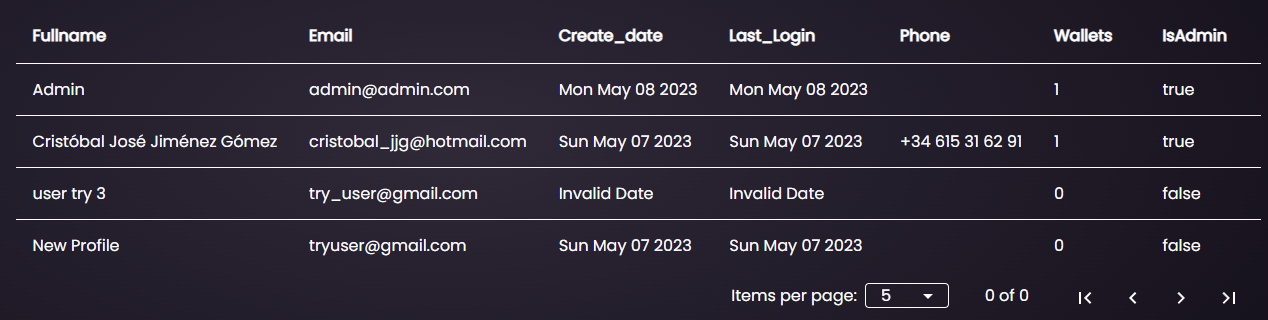
\includegraphics[scale=0.5]{./Ilustraciones/table-paginator.png}\\
    \textbf{Fuente:} Trabajo Propio en la zona de admin [\url{https://tft-galeria-nft-web3.vercel.app/admin/users}]
\end{figure}
\hfill \break